\documentclass[12pt]{article}
\usepackage{amsmath}
\usepackage{amssymb}
\usepackage{stackrel}
\usepackage{cite}
\usepackage{color}
\usepackage[margin=1in,footskip=0.15in]{geometry}
%\usepackage[]{algorithm2e}
\usepackage{algorithm}
% Need it for floating environment
\usepackage[noend]{algpseudocode}
% Hide endif .etc
\usepackage{caption}
% Need it for \caption*
\usepackage{xspace}
% Fix macro spacing bug
\usepackage[utf8]{inputenc}
\usepackage[english]{babel}
\usepackage{amsfonts}

\usepackage{tikz}
\usepackage{graphicx}
\usetikzlibrary{arrows}
\tikzset{every picture/.style={font issue=\scriptsize},
         font issue/.style={execute at begin picture={#1\selectfont}}}

%-------------------------------------------------------------
\usepackage{float}

\usepackage{algorithm}
\usepackage{algpseudocode} 

\algnewcommand\algorithmicinput{\textbf{Input:}}
\algnewcommand\Input{\item[\algorithmicinput]}

\algnewcommand\algorithmicoutput{\textbf{Output:}}
\algnewcommand\Output{\item[\algorithmicoutput]}

\algnewcommand\algorithmicparameters{\textbf{Parameters:}}
\algnewcommand\Parameters{\item[\algorithmicparameters]}
\renewcommand{\thealgorithm}{\arabic{algorithm}}

\algtext*{EndIf} % Remove "end if" text
\algtext*{EndFor} % Remove "end for" text
\algtext*{EndWhile} % Remove "end while" text
\algtext*{EndFunction} % Remove "end function" text

\renewcommand{\algorithmicrequire}{\textbf{Input:}}
\renewcommand{\algorithmicensure}{\textbf{Output:}}
\renewcommand{\algorithmicensure}{\textbf{Parameters:}}
%%----------------------------------------------------------
%%Macros:
\renewcommand{\j}{j} % index of single-cell
\newcommand{\CN}{C} %copy number (for haplotypes)
\newcommand{\X}{X} % read count
\renewcommand{\d}{d} % direction
\newcommand{\D}{\mathcal{D}} % direction set
\renewcommand{\k}{k} % index of the segment
\newcommand{\h}{h} % haplotype index
\renewcommand{\H}{\mathcal{H}} % haplotype set
\newcommand{\T}{T} % strand state random var
\newcommand{\V}{V} % variation (SV type)
\newcommand{\N}{N} % W and C CN in segment strand patterns
%%----------------------------------------------------------

\newtheorem{theorem}{Theorem}[section]
\newtheorem{definition}[theorem]{Definition}
\newtheorem{proposition}[theorem]{Proposition}

\title{Notations and the statistical model for read count of StrandSeq data}

\begin{document}

\maketitle

\section{Computing Strand-seq read count likelihoods based on a negative binomial (NB) model}

The read counts in genomic regions are shown to come from a Negative Binomial (NB) distribution \textcolor{red}{cite}. %TODO:FIXME~\citep{nb}.
Given a set of breakpoints and the estimated NB $p$ and $r$ parameters, we compute the likelihood of the observed Watson and Crick read counts per single-cell and segment for each haplotype-resolved SV status.

\subsection{Notations}
We present a set of notations in table~\ref{notations}. $\X$, $\T$ and $\V$ denote read counts and single-cell strand states and SV type, respectively.
Note that a haplotype-resolved SV class can be encoded as the number of normal and inverted copies of a region in each haplotype, which are denoted by $C$ notation.
$S$ denotes the size of a segment, which is defined as the number of bins inside the segment, and $N$ is the number of W and C copy numbers in a segment in a single-cell.

Note that segment strand pattern is differnt from single-cell strand states.
The latter is refered to the inherited strand-state in a single-cell in a chromosome, which can be variable in the range of a chromosome in case an SCE event happens, and it can only have one of the four possible states in $\{CC,CW,WC,WW\}$ for diploid cells, i.e., it can have $W$ or $C$ state in each haplotype.
However, segment strand pattern is a function of single-cell strand state and the SV class in a segment.
For example, if the strand state in a single-cell is $WW$ in a chromosome and an inverted duplication happens in a segment in that chromosome, the strand pattern in that segment will be $WWC$.
Table \textcolor{red}{S2} shows the values of segment strand patterns for different SV classes and single-cell strand states.

\subsection{Probabilistic model}
The Strand-seq directional read counts in segments are assumed to be generated by the following probabilistic model:
for each single-cell and each segment, the segment Watson and Crick copy number ($N$) is a function of the haplotype-specific single-cell strand state ($T$) and the SV class ($V$) in that segment. The strand pattern of segment $\k$ in single-cell $\j$ ($SP_{\j,\k}$) and the Watson and Crick copy numbers of the segment can be computed as follows:

\begin{align}\label{strand-pattern}
	&SP_{\j,\k,\h_1} = {\T^{\stackrel{\rightarrow}\CN_{\j,\k,\h_1}}_{\j, \k, \h_1}}.
				  {\overline{\T}^{\stackrel{\leftarrow}\CN_{\j,\k,\h_1}}_{\j, \k,\h_1}}\\
	&SP_{\j,\k,\h_2} = \T^{\stackrel{\rightarrow}\CN_{\j,\k,\h_2}}_{\j, \k, \h_2}.
				  {\overline{\T}^{\stackrel{\leftarrow}\CN_{\j,\k,\h_2}}_{\j, \k,\h_2}}\nonumber\\
	&SP_{\j,\k} = SP_{\j, \k, \h_1}.SP_{\j, \k, \h_2}\nonumber\\
	&\N_{\j, \k}^W = \text{number of W letters in } SP_{\j,\k}\nonumber\\
	&\N_{\j, \k}^C = \text{number of C letters in } SP_{\j,\k}\nonumber
\end{align}
where $\overline{\T}$ means the opposite direction for $\T \in \{W, C\}$, dot is the operation for concationating strings, and $\T^C$ means concatenation of $\T$ for $C$ times.

Given the Watson and Crick copy numbers in a segment, we can compute the likelihood of the observed read counts by NB distribution:
\begin{align}
	\X_{\j,\k}^W \sim NB(r_{\j,\k}^W, p)\nonumber\\
	\X_{\j,\k}^C \sim NB(r_{\j,\k}^C, p)\nonumber
\end{align}
where $p$ is the estimated $p$ parameter in NB distribution from bin read counts, and $r_{\j,\k}^W$ and $r_{\j,\k}^C$ are proportional to the estimated parameter $r_\j$, the segment size $L_\k$ and the Watson and Crick segment copy numbers ($\N_{\j, \k}^W$ and $\N_{\j, \k}^W$) and hence are computed as follows (for $d \in \{W,C\}$):
\[
r_{\j,\k}^d = 
\begin{cases}
\frac{1}{2}\alpha r_\j L_\k &\text{if } \N_{\j, \k}^d = 0 \\ 
\frac{1}{2}(1- \alpha) r_\j L_\k \N_{\j, \k}^d &\text{otherwise}
\end{cases}
\]
In this formula, $\alpha$ is a parameter in our model indicating the fraction of background reads that come from the opposite of the expected direction. These noisy background reads have been observed in Strand-seq data, which is the reason we incorporate this parameter in our model. Note that the $\frac{1}{2}$ coefficients in the above formula is for scaling the dispersion parameter to copy number 1 ($r_\j$ is defined for copy number 2).

To sum up, every haplotype-resolved SV class ($\V$) in a segment together with the haplotype-resolved strand state of a single-cell ($\T$), define a Watson and Crick copy number ($\N$), which will be then used to compute the NB likelihood of the observed read counts.


\begin{figure}
	\begin{center}
		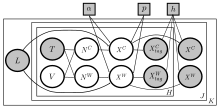
\includegraphics[width=\textwidth]{graphical_model_v2_haplotagged-equal-sized-circle}
	\end{center}
\caption{A plate notation representation of the graphical model for directional strand-seq read counts in genomic segments resulting from SV classes. Circles represent random variables, and squares show the model parameters. Gray and white objects show observed and latent (hidden) variables, respectively. $J$, $K$, and $H$ denote the set of single-cells, segments, and haplotypes. $\T_{\h,\k,\j}$ and $\V_{\h,\k,\j}$ respectively denote the strand state and the SV status of haplotype h in segment s in single-cell $\j$. $\N^W$ and $\N^C$ denote W and C copy numbers, and $\X^W$ and $\X^C$ denote W and C read counts, respectively. Note that the read counts are not observed (white circles inside the $H$ box) by their haplotypes, but they are observed with no haplotype information (white circles outside the $H$ box). A small fraction of the reads (determined by the heterozygosity parameter $h$) are observed by their haplotypes (tagged gray read count variables inside the $H$ box). $\alpha$ is the parameter showing the fraction of the background reads (noisy reads sampled from the opposite of the expected direction), and $p$ and $r$ are the $NB$ parameters, which are estmiated in mosaicatcher based on bin read counts.}
\end{figure}

\begin{table*}[tb]
	\caption{Overview of notations}
	\centering
	\begin{tabular}{  p{4cm} p{12.5cm} }
		\hline
		Notation & Definition\\
		\hline
		$\X_{\j,\k, \h}^W$ & The number of Strand-seq reads from single cell $\j$ and haplotype $\h$ mapped to the $\k$th segment in Watson direction\\

		$\X_{\j,\k, \h}^C$ & The number of Strand-seq reads from single cell $\j$ and haplotype $\h$ mapped to the $\k$th segment in Crick direction\\
		
		$\X_{\j,\k,\h,tag}^W$ & The number of Strand-seq reads from single cell $\j$  mapped to the $\k$th segment in Watson direction and tagged with haplotype $\h$\\
		
		$\X_{\j,\k,\h,tag}^C$ & The number of Strand-seq reads from single cell $\j$ mapped to the $\k$th segment in Crick direction and tagged with haplotype $\h$\\
		
		$\X_{\j,\k}^W$ & $\X_{\j,\k,\h}^W + \X_{\j,\k,\h}^W$\\
		
		$\X_{\j,\k}^C$ & $\X_{\j,\k,\h}^C + \X_{\j,\k,\h}^C$\\
		
		$\X_{\j,\k}$ & $(\X_{\j,\k}^W, \X_{\j,\k}^C)$\\
		
		$\T_{\j, \k, \h}$ & The strand state ($\in \{C,W\}$) of single cell $\j$ in haplotype $\h$ in the part of chromosome covering segment $\k$\\
		
		$\T_{\j,\k}$ & $\T_{\j, \k, \h_1}.\T_{\j, \k, \h_2}$\\
		
		$\stackrel{\rightarrow}{\CN}_{\j,\k,\h}$ & The number of copies of segment $\k$ in single-cell $\j$ and haplotype $\h$ \\
		
		$\stackrel{\leftarrow}{\CN}_{\j,\k,\h}$ & The number of inverted copies of segment $\k$ in single-cell $\j$ and haplotype $\h$ \\
		
		$\V_{\j, \k, \h}$ &$(\stackrel{\rightarrow}{\CN}_{\j,\k,\h}, \stackrel{\leftarrow}{\CN}_{\j,\k,\h})$ : SV type in segment $\k$ in single-cell $\j$ and haplotype $\h$\\
		
		$p$ & The $p$ parameter in NB distribution for the read counts from a single-cell inside a bin for normal copy number 2\\
		
		$r_\j$ & The dispersion ($r$) parameter in NB distribution for the read counts from single-cell $\j$ inside a bin for normal copy number 2\\
		
		$r_{\j,\k}^W$ & The dispersion ($r$) parameter in NB distribution for Watson read counts from single-cell $\j$ in segment $\k$\\
		
		$r_{\j,\k}^C$ & The dispersion ($r$) parameter in NB distribution for Crick read counts from single-cell $\j$ in segment $\k$\\
		
		$L_\k$ & size (number of bins) of segment $\k$\\
		
        $p_{\j, \k, \h}^W$ & Probability that a read from single-cell $\j$ and segment $\k$ is in Watson direction and tagged with haplotype haplotype $\h$\\
		
		$p_{\j, \k, \h}^C$ & Probability that a read from single-cell $\j$ and segment $\k$ is in Crick direction and tagged with haplotype haplotype $\h$\\
		
		$\N_{\j, \k, \h}^W$ & Watson copy number in single-cell $\j$ and segment $\k$ in haplotype $\h$\\
		
		$\N_{\j, \k, \h}^C$ & Crick copy number in single-cell $\j$ and segment $\k$ in haplotype $\h$\\
		
		$\N_{\j,\k}^W$ & $\N_{\j, \k, \h_1}^W + \N_{\j, \k, \h_2}^W$: Watson copy number in single-cell $\j$ and segment $\k$\\
		
		$\N_{\j,\k}^C$ & $\N_{\j, \k, \h_1}^C + \N_{\j, \k, \h_2}^C$: Crick copy number in single-cell $\j$ and segment $\k$\\
		
		$\N_{\j, \k}$ & $(\N_{\j, \k}^W, \N_{\j, \k}^C)$\\
		
		$SP_{\j,\k, \h}$ & $\in \{C,W,CC,WC,WW,CCC,CCW, \cdots\}$ : strand pattern of segment $\k$ in single-cell $\j$ in haplotype $\h$\\
		
		$SP_{\j,\k}$ & $SP_{\j, \k, \h_1}.SP_{\j, \k, \h_2}$\\
		\hline
	\end{tabular}
	\label{notations}\vspace{-4.5mm}
\end{table*}

\section{Computing haplotagged Strand-seq read count likelihoods based on a multinomial model}

MosaiCatcher phases a subset of SNPs by Strand-seq data using StrandPhaseR \textcolor{red}{cite} by exploiting the haplotype information in 'WC' regions/cells.
It can then tag the Strand-seq reads that cover phased SNPs by their haplotypes. The number of haplotagged Strand-seq reads in a segment/cell ($\X^C_{\j,\k,\h_1,tag}, \X^C_{\j,\k,\h_2,tag}, \X^W_{\j,\k,\h_1,tag}, \X^W_{\j,\k,\h_2,tag}$) are assumed to be the outcome of a multinomial distribution, the parameters of which are the probabilities of having a Strand-seq read in each of the four categories Crick/Watson read in haplotype $h_1/h_2$.

For each segment and cell, haplotype-specific strand pattern can be computed based on equation~\ref{strand-pattern} as a function of the strand state and SV class. The haplotype-specific strand pattern defines W and C copy numbers in each haplotype ($\N^C_{\j,\k,\h_1}, \N^C_{\j,\k,\h_2}, \N^W_{\j,\k,\h_1}, \N^W_{\j,\k,\h_2}$).
The probabilities of having a tagged read in each of these four classes (multinomial distribution parameters) are denoted by $p^C_{\j,\k,\h_1}, p^C_{\j,\k,\h_2}, p^W_{\j,\k,\h_1}$, and $p^W_{\j,\k,\h_2}$, which are simply proportional to their corresponding copy  numbers. We use a parameter denoted by $\alpha \in (0,1)$ to take into account any possible noise that leads to have a read in a wrong category. In other words, if any of the copy numbers in these four classes is zero, we set it's corresponding probability to $\alpha$. More precisely, we define the define the multinomial parameters and consequently compute the likelihood of the observed haplotagged read counts as follows (for $d \in \{W, C\}$ and $\h \in \{H_1, H_2\}$):
\begin{align}
	&p^d_{\j,\k,\h} \propto \max(\alpha, \N^d_{\j,\k,\h}) \\
	(\X^C_{\j,\k,\h_1,tag}, \X^C_{\j,\k,\h_2,tag}, \X^W_{\j,\k,\h_1,tag},& \X^W_{\j,\k,\h_2,tag}) \sim \nonumber Multinomial(p^C_{\j,\k,\h_1}, p^C_{\j,\k,\h_2}, p^W_{\j,\k,\h_1}, p^W_{\j,\k,\h_2})
\end{align}

\bibliographystyle{natbib}
% \bibliographystyle{achemnat}
% \bibliographystyle{plainnat}
% \bibliographystyle{abbrv}
% \bibliographystyle{bioinformatics}

\bibliographystyle{plain}

\bibliography{document}

\end{document}